\documentclass[10.9pt]{article}

\usepackage[paper=letterpaper,centering,margin=1.0in]{geometry}
\usepackage{setspace}

\usepackage[american]{babel}
\usepackage{epsfig,subfigure}
\usepackage{color,cite}
\usepackage{amsthm,amsfonts,amsmath,amssymb,amstext,latexsym}
\usepackage{multirow}
\usepackage{soul}
%\usepackage{xxcolor}
\usepackage{xcolor}
%\usepackage{hyperref}
\usepackage{algorithm}
\usepackage{algpseudocode}

\usepackage{graphicx}
\usepackage{amstext}

%\usepackage[utf8]{inputenc}
%\usepackage{enumitem}

%\algnewcommand{\IIf}[1]{\State\algorithmicif\ #1\ \algorithmicthen}
%\algnewcommand{\EndIIf}{\unskip\ \algorithmicend\ \algorithmicif}
\newcommand{\algorithmicbreak}{\textbf{break}}

\newcommand*{\Cdot}[1][1.25]{%
  \mathpalette{\CdotAux{#1}}\cdot%
}
\newdimen\CdotAxis
\newcommand*{\CdotAux}[3]{%
  {%
    \settoheight\CdotAxis{$#2\vcenter{}$}%
    \sbox0{%
      \raisebox\CdotAxis{%
        \scalebox{#1}{%
          \raisebox{-\CdotAxis}{%
            $\mathsurround=0pt #2#3$%
          }%
        }%
      }%
    }%
    % Remove depth that arises from scaling.
    \dp0=0pt %
    % Decrease scaled height.
    \sbox2{$#2\bullet$}%
    \ifdim\ht2<\ht0 %
      \ht0=\ht2 %
    \fi
    % Use the same width as the original \cdot.
    \sbox2{$\mathsurround=0pt #2#3$}%
    \hbox to \wd2{\hss\usebox{0}\hss}%
  }%
}


%\algdef{SE}[SUBALG]{Indent}{EndIndent}{}{\algorithmicend\ }%
%\algtext*{Indent}
%\algtext*{EndIndent}



\newcommand{\squishlist}{
 \begin{list}{$\bullet$}
  { \setlength{\itemsep}{0pt}
     \setlength{\parsep}{3pt}
     \setlength{\topsep}{3pt}
     \setlength{\partopsep}{0pt}
     \setlength{\leftmargin}{1.5em}
     \setlength{\labelwidth}{1em}
     \setlength{\labelsep}{0.5em} } }

\newcommand{\squishend}{
  \end{list}  }

\newtheorem{theorem}{Theorem}
\newtheorem{lemma}{Lemma}
\newtheorem{conjecture}{Conjecture}
\newtheorem{remark}{Remark}
% \newtheorem{proof}{Proof}
\newtheorem{proposition}{Proposition}
\newtheorem{observation}{Observation}
\newtheorem{definition}{Definition}
\newtheorem{corollary}{Corollary}
\newtheorem{assumption}{Assumption}

\newcommand{\bydef}{\stackrel{\rm{def}}{=}}
%\newcommand{\textul}[1]{\underline{#1}}

\newcommand{\cP}{{\cal P}}
\newcommand{\cR}{{\cal R}}
\newcommand{\cK}{{\cal K}}
\newcommand{\norm}[1]{\left\Vert#1\right\Vert}
\newcommand{\mc}[1]{\mathcal{#1}}
\newcommand{\Lrz}{\mbox{${\mathbb L}$}}
\newcommand{\DMU}{\text{DMU}}


% Comments colors conventions
\newcommand{\J}[1]{{\textcolor{cyan}{#1}}}
\newcommand{\JC}[1]{\textbf{{\textcolor{red}{Juan: #1}}}} 
\newcommand{\SAB}[1]{\textbf{{\textcolor{orange}{Sab: #1}}}} 

\newcommand{\preg}[1]{\textbf{{\textcolor{blue}{Sab: #1}}}} 


\def\R{\mbox{${\mathbb R}$}}           % Real numbers
\def\N{\mbox{${\mathbb N}$}}           % Natural numbers
\def\Z{\mbox{${\mathbb Z}$}}           % Integer numbers

\def\E{\mbox{${\mathbb E}$}}           % Expected value


\title{ Whisper Project \\ 
\begin{large} - Initial Report - }

\author{
\begin{center}
    \begin{tabular}[c]{  p{3.3cm}  p{3.3cm}  p{3.3cm} }
		Fernando Villa & Khalid Alobaid & Mariya Abdiyeva \\
		Nicolas Cabuli & Oluremi Obolo & Santiago Arrubla
    \end{tabular}
\end{center}
}



%\author{Fernando Villa \and Khalid Alobaid \and Mariya Abdiyeva \and Nicolas Cabuli \and Oluremi Obolo \and Santiago Arrubla}

\begin{document}
\date{7 Febraury 2017}
\maketitle


\section{Project Description}
\label{sec:part 1}

\subsection{Requirements (Aims)}

Our aim is to create a distributed chat system with the following specific requirements by  priority.

\begin{table}[ht]
\caption{Requirements by priority level}
\label{tab:requirements}
    \begin{tabular}[c]{ | p{5cm} | p{5cm} | p{5cm} |}
		\hline
		\centering\textbf{Priority 1} & \centering{\textbf{Priority 2}} & \centering\textbf{Priority 3} &
    \hline
    \parbox[t]{5cm}{-Secure connection\\-Encrypted messages\\ -iOS, Android and Web platforms (at least two platforms)\\ -Contact list\\ -Search for contacts\\ -Sign in by email or Gmail \\ -One to one conversation (text message)} &  \parbox[t]{5cm}{-Send images\\ -Group chat\\ -Chat bubbles instead of username\\ -Notifications of received messages}
& \parbox[t]{5cm}{-Sign Up with Facebook\\ -Availability to send other type of media (e.g. video, voice notes, etc.)\\ -Online status of other users\\ -Acknowledgment of received, delivered and read messages, including date time\\ -Ability to use the chat offline}\\
    \hline
    \end{tabular}
\end{table}


\subsection{Strategy and Timetable}

Our strategy is to develop three client-based platforms (i.e. Android, iOS and Web) using Firebase as a server. The reason for including a third platform is to act as a backup should there be problem with any of the platforms during testing which we are unable to debug at the end. The tentative timetable (Figure ~\ref{fig:timetable}) presents the main activities required to complete our final product. It is important to state that the timetable and our strategy is constructed based on the Scrum ~\cite{scrum} methodology, which  is an agile software development guide that allows us to iterate and make incremental and evolutionary contributions.  We will also use different Project Management roles like a Scrum Master (who removes team obstacles and pushes resolutions) and the product owner (who acts as the client voice) to ensure a high-quality product. The main activities are explained as follows: 

\begin{enumerate}
	\item \textbf{Plan}: Here we defined how we are going to work, our goals and organization as a team. We also discussed our individual strengths and weaknesses and the tools available to achieve our aim and objectives.
	\item \textbf{Firebase}: For simplicity, costs (free) and security we are using this Backend as a Service platform to have a robust system which takes care of the authentication, rules for accessing the database (read/write) and the storage of documents so that we could focus on the core functionality, i.e. the actual messaging.
	\item \textbf{UI}: Refers to designing the User Interfaces for all the clients.
	\item \textbf{Client Development}: This is the development of the specific application for each type of client (Android, iOS and Web): 
	\begin{enumerate}
		\item \textbf{Setup}: Here we add the required files and initialize the repository on GitHub. Then we create the project on Firebase so that we could share the same API Keys.
		\item \textbf{Login}: Build the login page, authentication using email and password, Gmail and Facebook if possible.
		\item \textbf{Conversations}: Text messaging between clients using Firebase as a central database containing the messages between recipients and taking care of the encryption. Add chat bubbles, send and receive messages, show them in an organized manner with timestamps.  
		\item \textbf{Image Message}: Share images inside messages (nice to have).
	\end{enumerate}
		\item \textbf{Integration Testing}: Test functionality across platforms. 
		\item \textbf{Quality Assurance}: Check that all clients communicate with the backend as intended in order to ensure that we cover all the required functionalities and fix any problem that we may have.	
\end{enumerate}

\begin{figure}[ht]
%[Parzen Window Estimated Distributions]
\centering
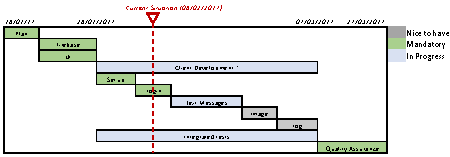
\includegraphics[width=0.9\textwidth]{figs/Timetable}
	\caption{Timetable}
	\label{fig:timetable}
\end{figure}


Please note that our activities in the client development are organized by hierarchy over time. Thus, developing the text message functionality (which is mandatory) is more important than the image message functionality (which is optional but highly desirable). Consequently, we decomposed our activities into tasks and allocated them to each team member as follows:

\begin{figure}[ht]
%[Parzen Window Estimated Distributions]
\centering
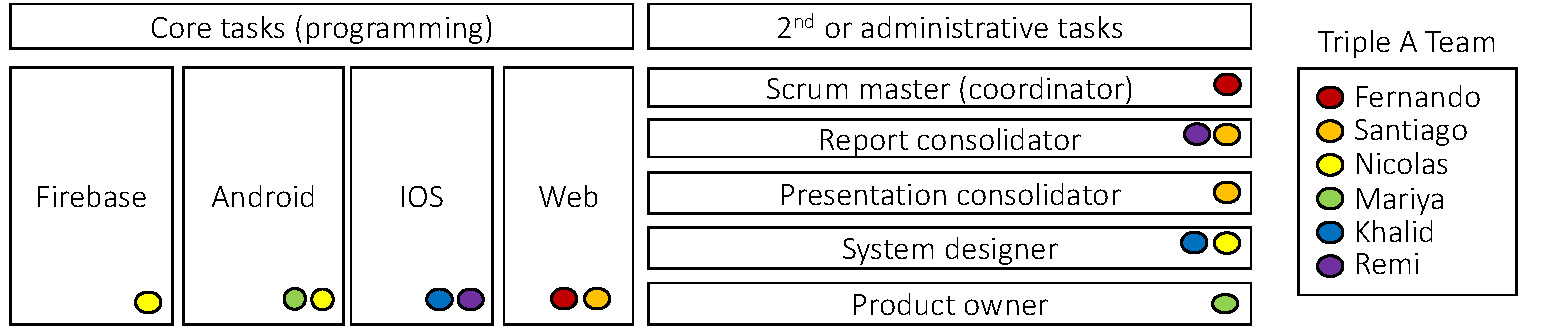
\includegraphics[width=1\textwidth]{figs/tasks}
	\caption{Tasks allocation}
	\label{fig:Tasks}
\end{figure}

\subsection{Current State}
Currently, we have developed the authentication functionality inside the three clients. Firebase authorizes the logged users and allows them see the data only if they are logged in.

\subsection{Next Steps}
Following our timetable, we are going to focus on making the proper database structure (chats, messages, users, receiver, sender, type of message, etc), rules for accessing the data inside the database (only user x and user y can see their own conversation) and adding new data to the database.

\section{Project Organization}
\label{sec:part 2}
Chat applications are around our daily lives. Most of the people don't get out of their homes without checking Facebook Messenger or Whatsapp. Other popular examples, just to mention a few, are chats like Slack, Telegram, Skype, Snapchat and Viber, among many others.

We did research about the most important programming trends and the clients available for the most popular applications. We used Stack Overflow Developer Survey in 2017 ~\cite{DeveloperStackoverflow} as a source, it establishes that the most popular technologies are Android, iOS and Web. In addition, the market share of iOS and Android in 2016 is about 12.9 and 86.2 percent, respectively ~\cite{DeveloperStackoverflow}.  We also added the Web client because web development has always been attractive for us, since companies like Google, Amazon and Facebook started from there. In addition, the entry barrier in a web application is lower than other developing environments.

One of the most important reviews we research at the beginning was proper methodologies to work as a group. Specifically, the agile methodology, proposed by Alistain Cockburn and Jim Highsmith ~\cite{rury346} was our first approach. However, the lack of experience set in and we didn't know how to tackle in advance many of the software challenges laying ahead. Moreover, the proper division of each single task of our software made us struggle at some point, and we  returned to the foundations of the agile methodology. That is, using an hybrid approach on which some tests were conducted at the end and others in each single iteration. In other words, our main challenge in this point was deciding how to tackle each part of the overall system and make the integration. 

As part of the creation of this project, we ultimately decided that in order to get the most out of it, we needed to learn more about different tools. We wanted to pick a challenging technology with the robustness needed but also with vasts amounts of information on the Internet and in books to try and reduce accelerate our learning curve the most we could to mitigate our knowledge lack. 

For the clients we decided to go with Android, iOS and Web and Firebase as our back-end because we were thinking of focusing on the User Experience inside the clients. We wanted users to have a good experience using our service and convince them to use it. From the beginning, we knew that the Authentication is a strong feature in Firebase. It allows us to control who can read your data and also let us select different services such as Facebook, Gmail, GitHub, and others to register and login. One of the main things we found that Firebase has is the real time database. Thanks to this feature, we could see all messages in real time in all the clients. 

As we mentioned before, Firebase was the best choice for our intended purposes, not only because is supported by Google. Aside all the benefits such as Web Analytics, Push Notifications, File storage, and the main reason, the price (which is free for our needs) and also support scalable applications. Firebase gives the flexibility to do a lot of ``back-end" code in the client side. Even though, it leverages a lot to the client, we realised this was interesting to test new ways of developing applications, as we only knew the basics around Object Oriented Programming. It gave us also the flexibility to focus on the front-end development but with the possibility to con troll features that normally a back-end covers. Another of the main reasons why we choose Firebase is that it has a good written documentation on its website. Lastly, it takes minimum setup to begin developing, which was a key point for us as we wanted to finish the project on time while competing between studies and time. Even with this concern in mind we had some challenges finishing it but we have learn a lot in this process.





\bibliography{references}
\bibliographystyle{plain}
\end{document}
